\documentclass{beamer}
\usepackage[ngerman]{babel}
\usepackage[utf8]{inputenc}
\usepackage{graphicx}
\usepackage{verbatim}
\usepackage[final]{listings}
\usepackage{multicol}

\lstset{language=bash}
\lstset{basicstyle=\ttfamily\small\mdseries}
\definecolor{darkgrey}{rgb}{0.95,0.95,0.95}
\definecolor{darkgreen}{rgb}{0.3,0.6,0.3}
\definecolor{darkred}{rgb}{0.8,0.2,0.2}
\definecolor{darkblue}{rgb}{0.1,0.15,0.85}
%\lstset{backgroundcolor=\color{darkgrey}}
\lstset{stringstyle=\color{darkred}}
\lstset{numberstyle=\color{darkgreen}}
\lstset{commentstyle=\color{darkgreen}}
\lstset{keywordstyle=\color{darkblue}}
\lstset{linewidth=\textwidth, showstringspaces=false}
\lstset{captionpos=tb}
\lstset{tabsize=1}
\lstset{breaklines=true}
\lstset{breakatwhitespace=true}
\lstset{morekeywords={git}}
\lstset{numbers=left}
\lstset{float=htb}
\lstset{numberstyle=\ttfamily\tiny}
\lstset{numbersep=10pt}

\usetheme{Singapore}
\usecolortheme{crane}

\title{git}
\author{Johannes Held}
\date{10.05.2010}

\begin{document}

\frame{\titlepage}

\frame{\tableofcontents}

\section{DVCS}
\frame{
	\frametitle{DVCS}
	\begin{itemize}
	\item verteilt
	\item schnell
	\item unabhänig
	\pause
	\item git, mercurial, bzr, monotone, darcs, uvm.
	\end{itemize}
}

\subsection{workflows}
\frame{
	\frametitle{workflows - zentralisiert}
	\begin{figure}[h]
		\center
		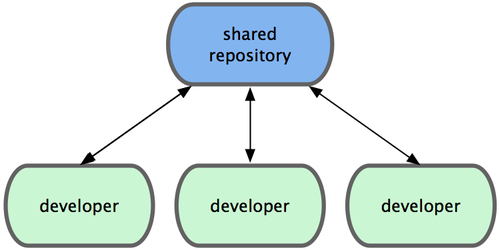
\includegraphics{pics/workflow_01.png}	
	\end{figure}
}

\frame{
	\frametitle{workflows - integriert}
	\begin{figure}[h]
		\center
		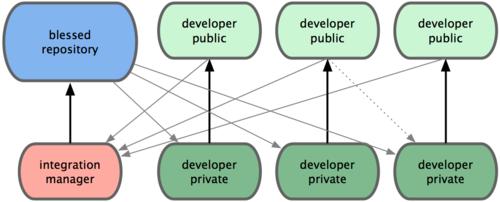
\includegraphics{pics/workflow_02.png}	
	\end{figure}
}

\frame{
	\frametitle{workflows - diktatur}
	\begin{figure}[h]
		\center
		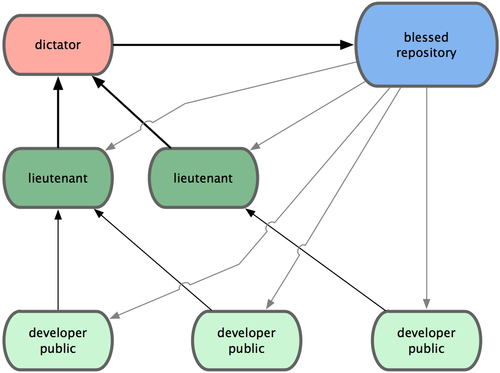
\includegraphics{pics/workflow_03.png}	
	\end{figure}
}

\section{git}
\frame{
	\frametitle{git}
	\begin{block}{O-Ton Linus Torvalds}
	DVCS are cool.\\
	You're an idiot if you're not using git!\\
	\small{http://www.youtube.com/watch?v=4XpnKHJAok8}	
	\end{block}
}

\subsection{init and commit}
\frame{
	\frametitle{init}
	\pause
	\lstinputlisting{listings/init.sh}	
}

\frame{
	\frametitle{staging}
	\pause
	\lstinputlisting{listings/stage.sh}
}

\frame{
	\frametitle{staging - split}
	\pause
	\lstinputlisting{listings/split.sh}	
}

\subsection{branch}
\frame{
	\frametitle{branch}
	\begin{figure}[h]
		\center
		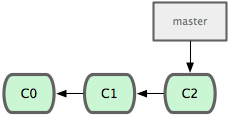
\includegraphics{pics/branch_01.png}	
	\end{figure}
}


\frame{
	\frametitle{branch}
	\begin{figure}[h]
		\center
		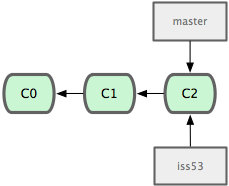
\includegraphics{pics/branch_02.png}	
	\end{figure}
}

\frame{
	\frametitle{branch}
	\begin{figure}[h]
		\center
		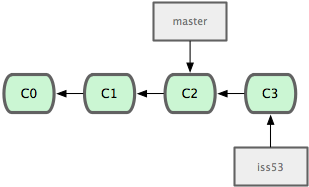
\includegraphics{pics/branch_03.png}	
	\end{figure}
}

\frame{
	\frametitle{branch}
	\begin{figure}[h]
		\center
		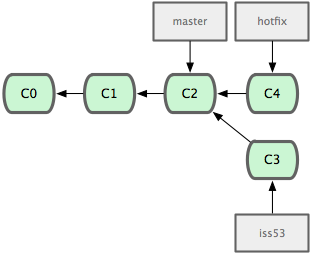
\includegraphics{pics/branch_04.png}	
	\end{figure}
}


\subsubsection{tracked remnote branch}
\frame{
	\frametitle{tracked remote branch}
	\begin{block}{checkout tracked remote branch}
		\lstinputlisting{listings/tracked_branch.sh}
	\end{block}
	\begin{block}{pull, push and delete}
		\lstinputlisting{listings/pull_push_del_tb.sh}
	\end{block}
}

\subsection{merge}
\frame{
	\frametitle{merge}
	\begin{figure}[h]
		\center
		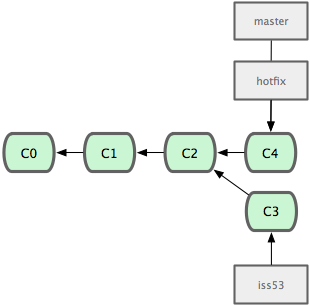
\includegraphics{pics/merge_01.png}	
	\end{figure}
}

\frame{
	\frametitle{merge}
	\begin{figure}[h]
		\center
		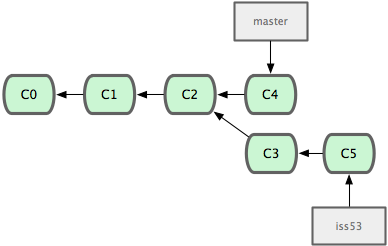
\includegraphics{pics/merge_02.png}	
	\end{figure}
}

\frame{
	\frametitle{merge}
	\begin{figure}[h]
		\center
		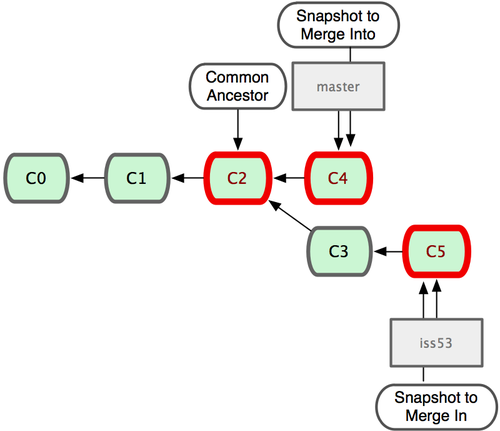
\includegraphics{pics/merge_03.png}	
	\end{figure}
}

\frame{
	\frametitle{merge}
	\begin{figure}[h]
		\center
		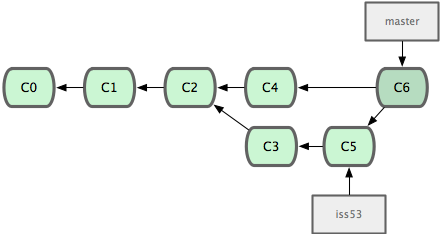
\includegraphics{pics/merge_04.png}	
	\end{figure}
}

\subsection{rebase}
\frame{
	\frametitle{rebase}
	\begin{figure}[h]
		\center
		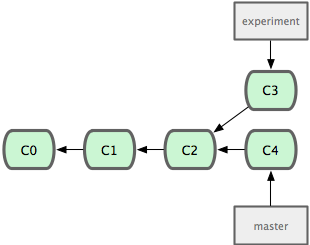
\includegraphics{pics/rebase_01.png}	
	\end{figure}

}

\frame{
	\frametitle{rebase}
	\begin{figure}[h]
		\center
		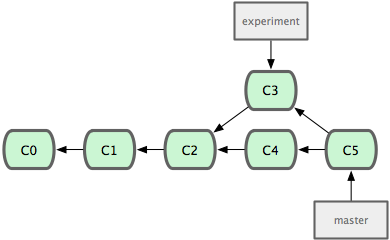
\includegraphics{pics/rebase_02.png}	
	\end{figure}

}

\frame{
	\frametitle{rebase}
	\begin{figure}[h]
		\center
		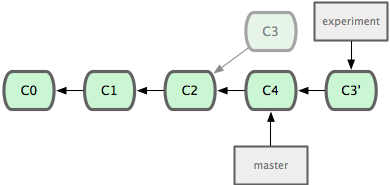
\includegraphics{pics/rebase_03.png}	
	\end{figure}

}

\frame{
	\frametitle{rebase}
	\begin{figure}[h]
		\center
		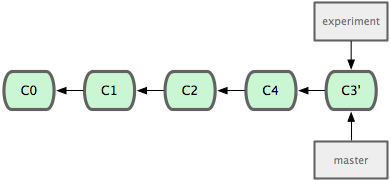
\includegraphics{pics/rebase_04.png}	
	\end{figure}

}

\section{diff to others like hg}
\frame{
	\frametitle{diff }
}

\section{Mehr Informationen}
\frame{
	\frametitle{Mehr Informationen}
	\begin{block}{Webseiten}
		 http://whygitisbetterthanx.com/
		\\ http://progit.org
		\\ \small{http://versioncontrolblog.com/comparison/Git/Mercurial/index.html}
		\\ http://www.gitready.com/
		\\ http://git-scm.com/
	\end{block}

	\begin{block}{Dieser Foliensatz}
		git clone git://github.com/hehejo/NTDM-GIT.git
	\end{block}
}


\end{document}
